
\begin{minipage}[t]{.6\linewidth}
	Le programme ci-contre (programme 1) a été écrit avec le logiciel Scratch.

\begin{enumerate}
  \item En prenant $C=50$ et $1 \mathrm{~cm}$ pour 10 pixels, tracer la figure construite en utilisant le \textit{Programme 1}.

  \item Quelle est la nature de la figure tracée? Justifier la réponse.

  \item On écrit le programme 2 en utilisant le bloc précédent, afin d'obtenir la figure représentée ci-après.
  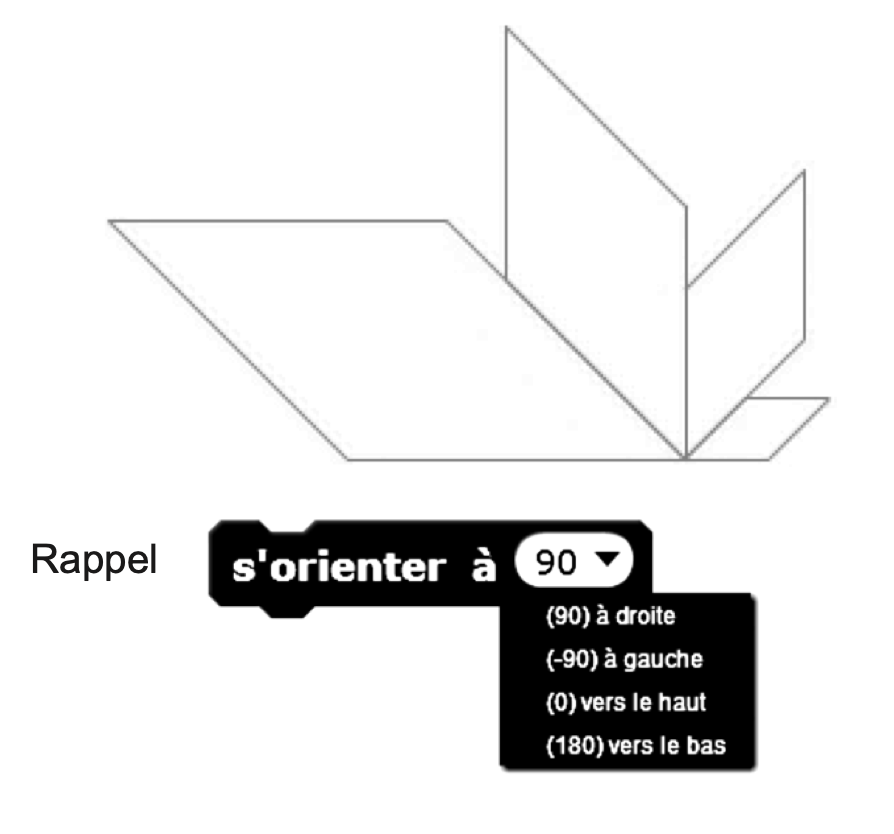
\includegraphics[width=.8\linewidth]{2022-g1-ex4-img2.png}
  
	\begin{enumerate}
		\item Quelles valeurs attribuer aux lettres $A$ et $N$ dans le \textit{programme 2} pour obtenir la figure correspondante ?
		\item Quelle est la valeur de la variable $\mathrm{C}$ une fois le programme exécuté ?
	\end{enumerate}

\item Comment peut-on modifier le \textit{programme 2} pour obtenir la figure ci-contre pour laquelle chaque segment mesure 30 pixels ?

	\centering
	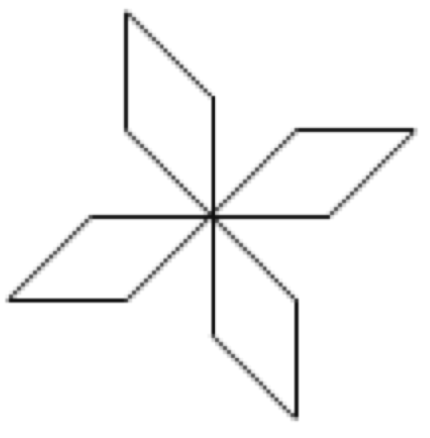
\includegraphics[width=.5\linewidth]{2022-g1-ex4-img3.png}
\end{enumerate}

\end{minipage}
\begin{minipage}[t]{.4\linewidth}
    \vspace{0cm}
	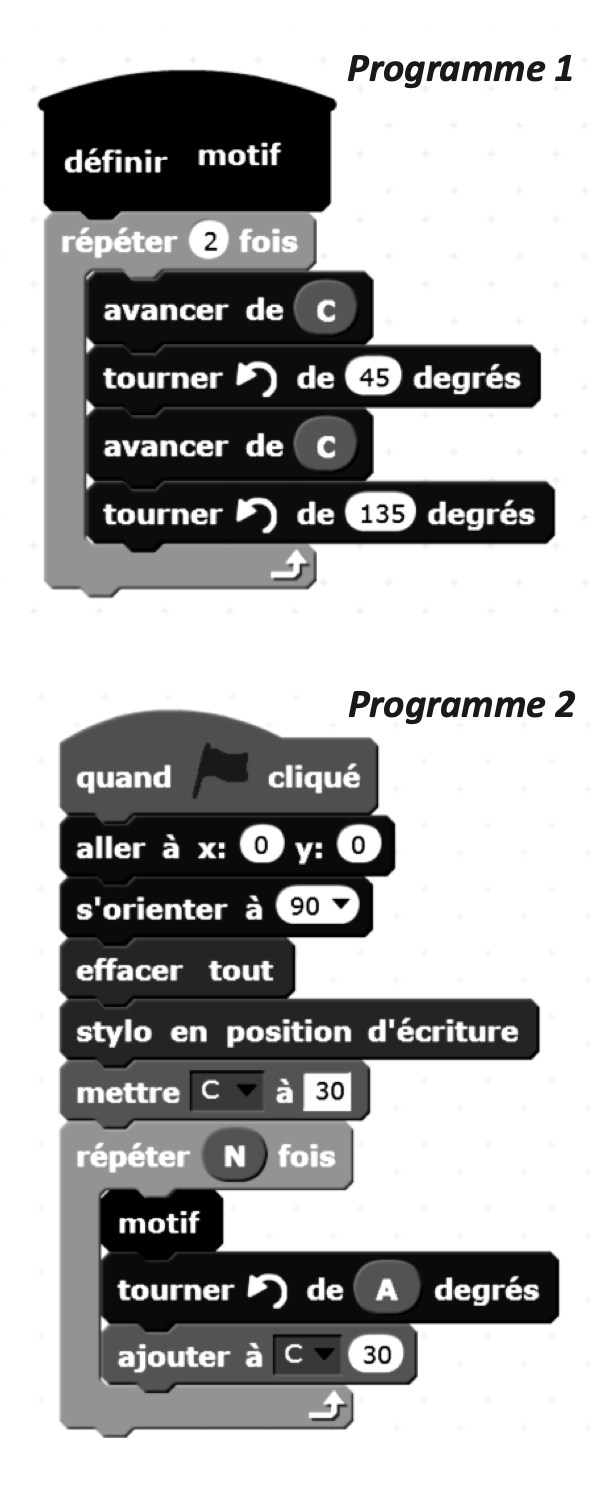
\includegraphics[width=\linewidth]{2022-g1-ex4-img1.png}
\end{minipage}

